\documentclass{report}

\usepackage[usenames,dvipsnames]{color}
\usepackage{xcolor}
\usepackage{listings}
\usepackage{caption}
\usepackage{courier}
\usepackage{fancyvrb}
\usepackage{xparse}
\usepackage{fullpage}
\usepackage{colortbl}
\usepackage{graphicx}
\DefineShortVerb{\|}
\DeclareCaptionFont{white}{\color{white}}
\DeclareCaptionFormat{listing}{\colorbox{gray}{\parbox{\textwidth}{#1#2#3}}}
\captionsetup[lstlisting]{format=listing,labelfont=white,textfont=white}
\lstset{language=Python, basicstyle=\ttfamily, showstringspaces=false,showspaces=false}
\lstdefinestyle{numbers}{numberstyle=\tiny}
\renewcommand*\arraystretch{1.75}
\NewDocumentCommand \method{ m m g g g g g g g }{%
	{\tt{\textcolor{red}{#1} #2(}%
		\IfValueTF{#3}{\textcolor{blue}{#3}%
			\IfValueTF{#4}{\textbf{,}\textcolor{blue}{#4}%
				\IfValueTF{#5}{\textbf{,}\textcolor{blue}{#5}%
					\IfValueTF{#6}{\textbf{,}\textcolor{blue}{#6}%
						\IfValueTF{#7}{\textbf{,}\textcolor{blue}{#7}%
						}{\tt{)}}%
					}{\tt{)}}%
				}{\tt{)}}%
			}{\tt{)}}%
		}{\tt{)}}%
	}%
}

\definecolor{lightblue}{rgb}{0.9,0.9,0.9}
\definecolor{lightyellow}{rgb}{0.95,0.95,0.95}
\graphicspath{ {./screenshots/} }


\begin{document}
\newcolumntype{b}{>{\columncolor{lightblue}}c}
\newcolumntype{y}{>{\columncolor{lightyellow}}l}

\begin{titlepage}
	\begin{center}
		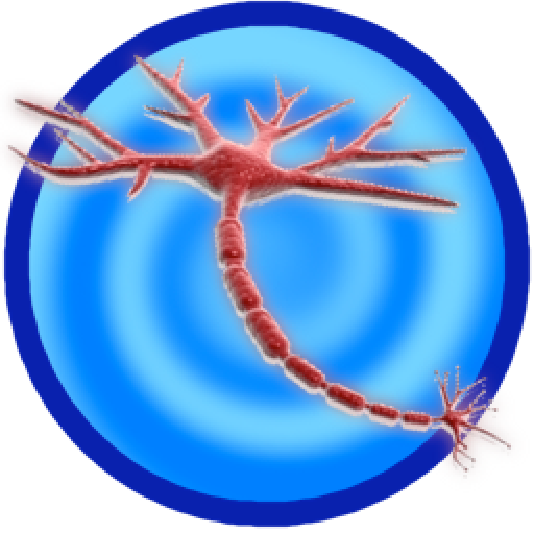
\includegraphics[width=0.35\textwidth]{icon.pdf}\\
		[4.0cm]
		\hrule\vspace{0.4cm}
		{ \huge \bfseries SpikeDB Version 1.1 User Manual }\\[0.4cm]
		\hrule 
		\vspace{4cm}
		\textsc{\LARGE McMaster University}\\
		[0.5cm]
		\textsc{\Large Written by Brandon Aubie}\\
		\vspace{0.5cm}
		{\large brandon@aubie.ca}

	\end{center}
\end{titlepage}

\tableofcontents 

\chapter{Introduction}
\begin{figure}[h]
\begin{center}
	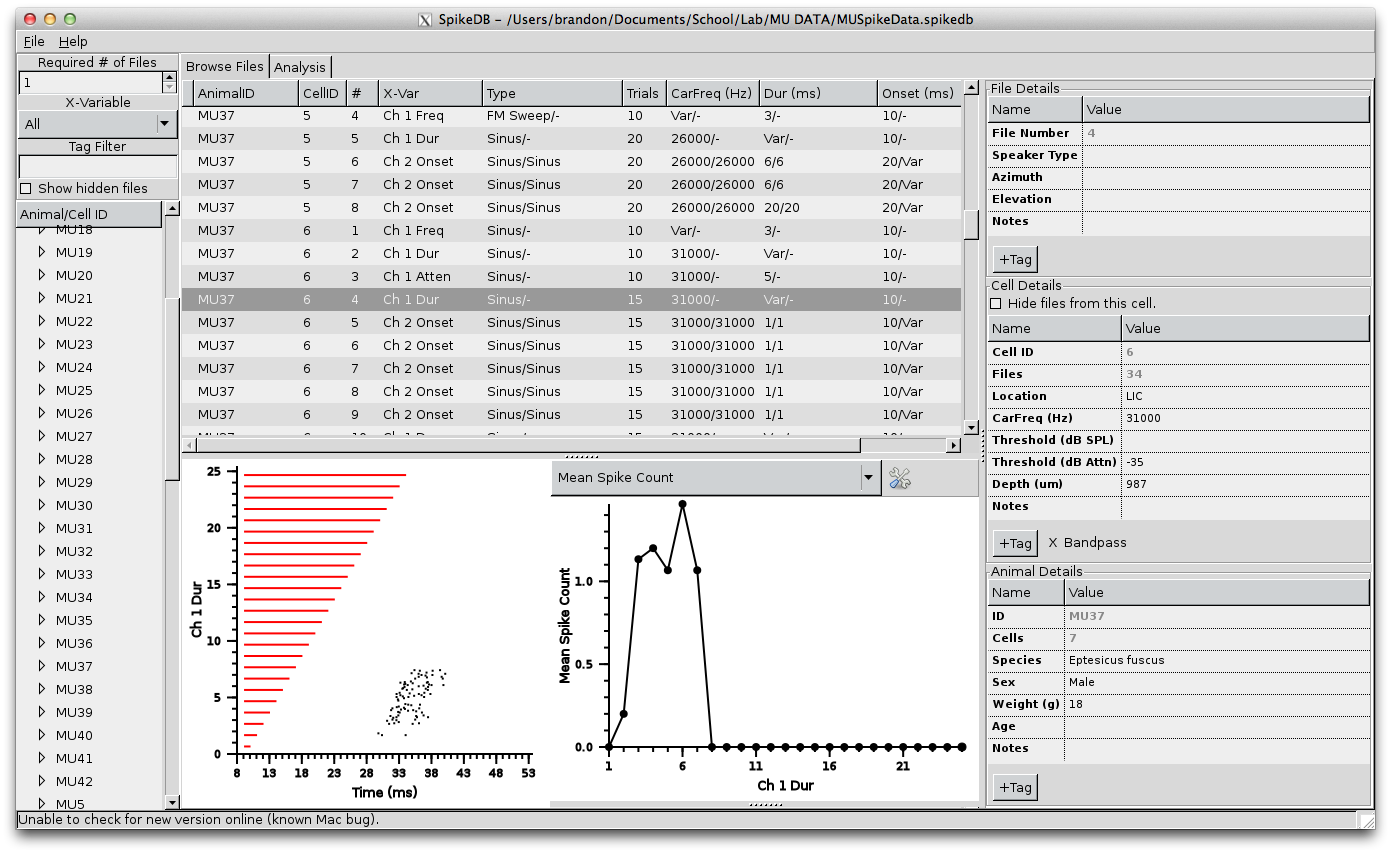
\includegraphics[width=0.5\textwidth]{main_window.png}
\end{center}
\caption{Main SpikeDB window showing a spike raster and mean spike count analysis plot.}
\end{figure}
SpikeDB is a database and analysis tool for electrophysiological recordings done with SPIKE (written by Brandon Warren). It runs on Linux and Mac OS X and Windows. The purpose of SpikeDB is to provide electrophysiologists with the ability to easily catalogue their electrophysiological recordings for future analysis. Animals, Cells, and Files can be assigned meta data such as tags to make finding them easier. Furthermore, all data becomes available in an embedded Python scripting interface to allow for powerful data analysis without the need to manually export and manipulate the data from SPIKE.


\clearpage
\chapter{User Interface}
\begin{figure}[h]
\begin{center}
	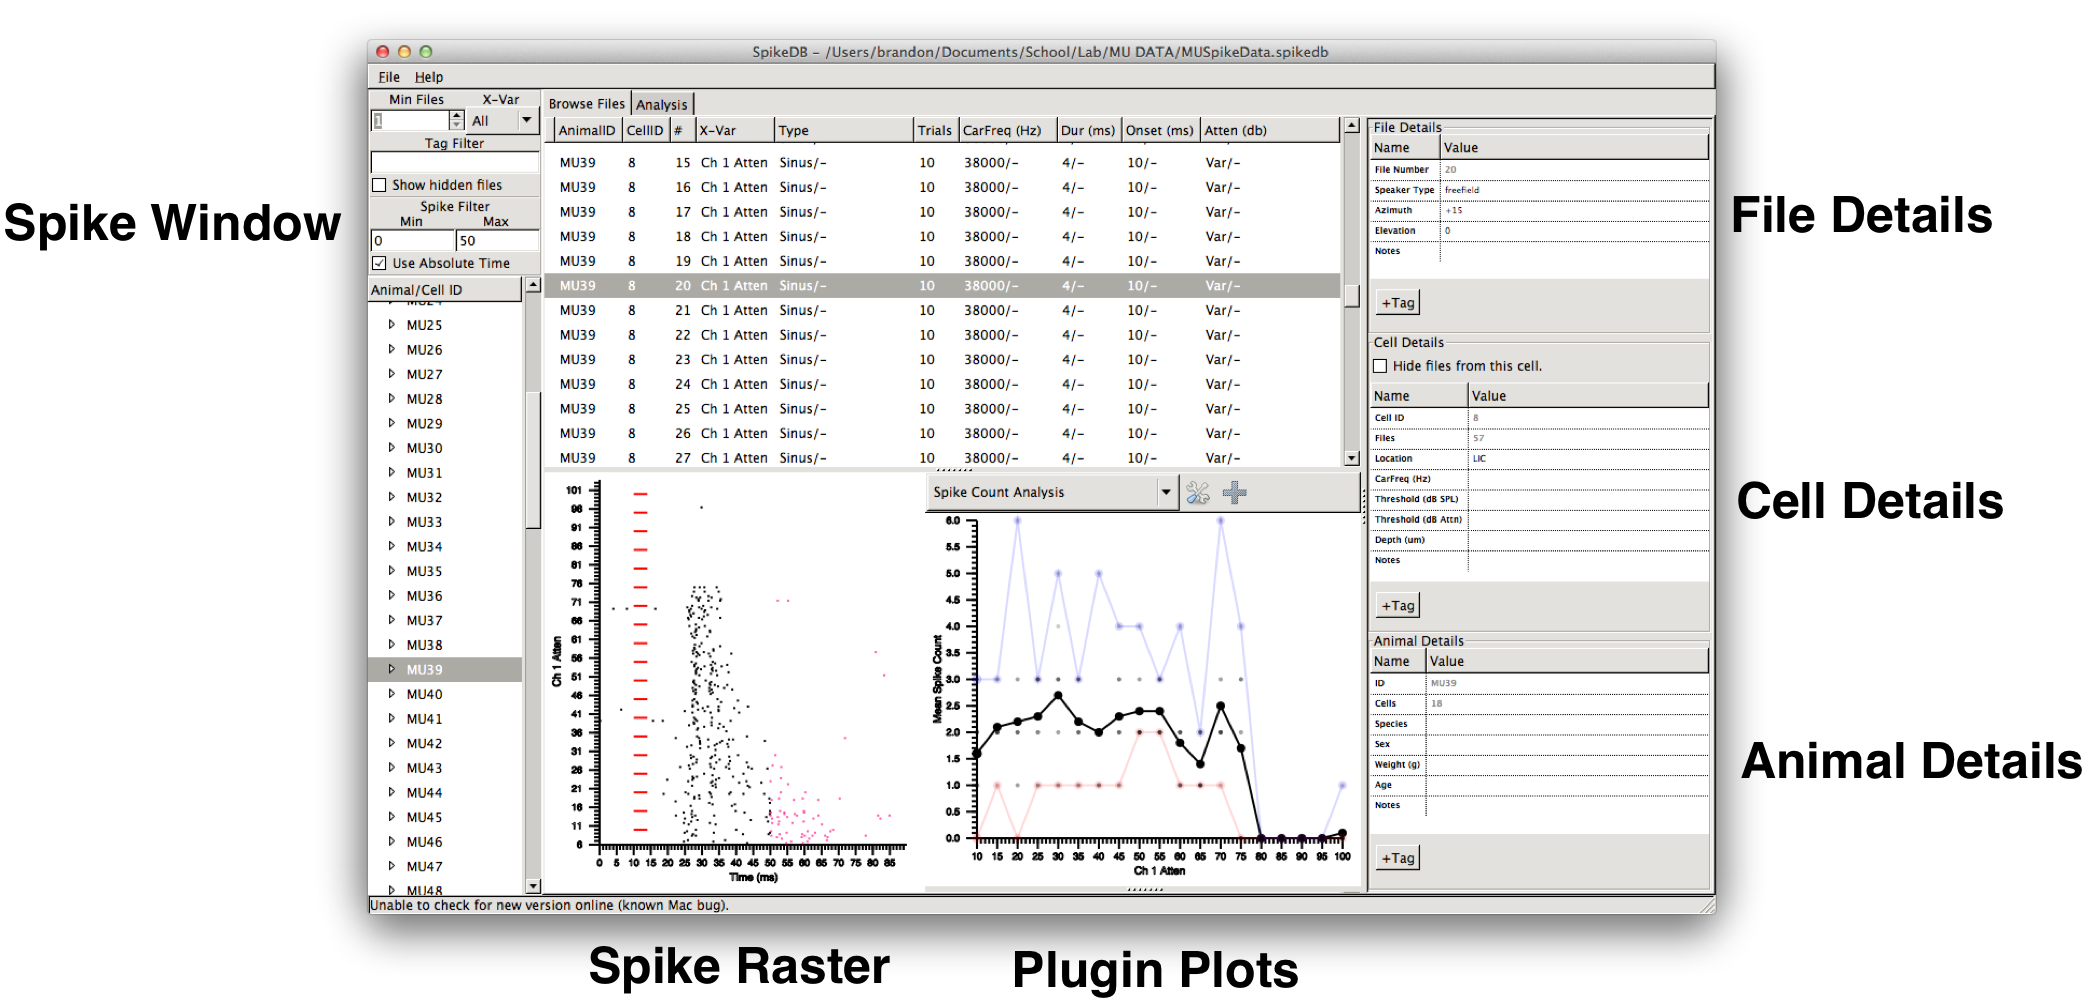
\includegraphics[width=0.6\textwidth]{main_window_letters.png}
\end{center}
\end{figure}
\begin{itemize}
	\item[A)] Filter Panel - Filter the files shown in the Browse Files list.
	\item[B)] Animal List - List of animals and cells currently imported.  Select an animal or a cell by selecting the arrow head next to each item. Only the selected animals or cells appear in the Browse Files list. Select |All Animals| to display all animals, cells and files in the Browse Files list.
	\item[C)] Browse Files list - A list of files currently selected and filtered.
	\item[D)] Spike Raster Plot - Displays each spike as a black dot and each stimulus as a line (red = Channel 1, blue = Channel 2).
	\item[E)] Quick Analysis Plot - Displays results of analysis script selected in the drop-down box or a custom script selected with the |Open| button in its toolbar.
	\item[F)] Animal Details Panel - Displays animal details of the currently selected file and allows the entry of custom data.
	\item[G)] Cell Details Panel - Displays cell details of the currently selected file and allows the entry of custom data.
\end{itemize}

		
\clearpage
\section{Importing Spike Data}
SpikeDB uses a database file (SQLite) to store spike data. This means that your SPIKE files are not modified in any way. Before viewing your SPIKE data in SpikeDB you must create a new database file and then import the spike files.
\begin{enumerate}
	\item First select the |Create New Database| option in the file menu. This file can be named anything and saved anywhere. For example you could name it |MySpikeData.db|. If multiple people need to access this data you could store it on a shared network drive.
	\item Click the |Save| button to create your new database file.
	\item  Next, select the |Import Spike Files| option form the file menu and select the directory where your SPIKE files are located. The import tool will go one level deeper than the directory you select if needed.  Therefore, you could have your SPIKE files in subdirectories of the directory you choose here.
	\item Click the |Open| button after you have chosen the directory with SPIKE files to automatically import them into SpikeDB. If you have already imported a file, SpikeDB is smart enough to recognize the duplicate and skip over that file.
\end{enumerate}


\section{Browse Files List}
To view a spike raster and quick analysis plot, click on any file in the list. Multiple files can be analyzed at the same time by selecting multiple files simultaneously (holding down CTRL on most computers while selecting files or hold down SHIFT to select a range of files). If a file is considered to be useless (incomplete recording or incorrect settings for example) then the file can be hidden from view by right clicking on it, selecting |View Details| and then checking the |Hide file in file list| checkbox.  As long as the |Show hidden files| checkbox in the filter panel is not checked, this file will not be displayed. The file details window also shows the time when the file was created.

\section{Filter Panel}
The filter panel is used to filter the files shown in the Browse Files window. This can be useful when browsing your data or when running analysis scripts.

\subsection{Required Number of Files}
Often we are only interested in cells with at least a minimum dataset and thus cells with only 1 or 2 files recorded are useless. Setting this value to a number greater than 1 will hide any cells that have less than that number of files recorded for it.

\subsection{X-Variable}
Use this drop-down to filter which types of files are shown based on the file's X variable.

\subsection{Tag Filter}
Animals and Cells and be given tags in their respective details panels on the right of the window. Only files that belong to an animal or a cell containing the tag entered in this window they will be shown in the Browse Files list. Leave blank to not filter on tags.

\subsection{Show hidden files}
Turn this option on to show files in the Browse Files list even if they have been manually marked as hidden. The hidden files will be tagged with an |H| to the left of the list when shown.

\section{Plots}
\subsection{General Usage}
\begin{itemize}
	\item \textbf{Zoom} - Left click and drag horizontally to zoom in on a subsection of data.  
	\item \textbf{Export Data} - Right click anywhere on the plot to bring up the options menu and select |Export Data|. This allows you to export the plotted data in CSV files that are ready for import into Excel or for use in other graphing software such as GLE.
\end{itemize}

\subsection{Spike Raster}
The spike raster is a built-in plot that displays the stimuli as red (channel 1) and blue (channel 2) lines and spikes as black dots. Zooming in on this plot will limit the spike times available to the Quick Analysis plot on the right.

\subsection{Quick Analysis}
By default, this plot will display the mean number of spikes per trial. Other analysis plugins are available in the drop down box or additional plugins can be loaded by clicking the |Open| icon. Generally, it is wise to use plugins that operate on selected files only here as no text display is available. For more general analysis on many files use the Analysis tab. That said, if multiple files of the same type are selected, the plots can be overlaid for easy comparison. Turn on the |Show Error Bars| option to display the error bars in graphs (generally shown as standard deviation).



\chapter{Analysis Plug-In Module}
\section{Basic Usage}
The Analysis Plug-In Module allows you to use the Python scripting language write custom analysis routines on one or many Spike recording files. Each Python script will have the |SpikeDB| object available to it.  This object provides access to all of the data held within SpikeDB as well as a host of methods useful for analysis.

\subsubsection{Quick Analysis Plugins}
Several Quick Analysis plugins are included with SpikeDB, however, it is easy to add your own. Quick Analysis plugins are shown in the drop-down box on the Quick Analysis and Analysis toolbars and are defined by scripts located in the plugins/ folder of the SpikeDB application. The location of this folder depends on your operating system. Refer to Table \ref{tblPluginLocations} for details.
\begin{table}[h]
	\begin{center}
	\caption{Default plugins folder locations on different operating systems.}
	\begin{tabular}{by}
		Microsoft Windows & C:\textbackslash Program Files\textbackslash SpikeDB\textbackslash plugins\textbackslash \\
		\hline
		Mac OS X & /Applications/SpikeDB.app/Contents/Resources/plugins/ (built-in) \\
		\emph{or} & /Library/Application Support/plugins/ (user added)\\
		\hline
		Linux & /usr/share/SpikeDB/plugins/ \\
	\end{tabular}
	\label{tblPluginLocations}
	\end{center}
\end{table}
Quick Analysis plugins function exactly the same way as other Analysis plugins with two minor differences. First, the name of the plugin to display in the toolbar drop-down list must be specified on the first line with three |#| symbols in the format 
\begin{center}|### Name Goes Here|\end{center}
Second, when retrieving files with the |getFiles()| method you will generally always want to pass |True| as the parameter to ensure that only the currently selected file(s) will be analyzed. When adding new Quick Analysis plugins to the plugins folder you must restart SpikeDB for them to be available in the drop-down list.

\section{Reference}
All functions listed in this section are accessed via the SpikeDB object.  For example, |SpikeDB.getFiles(True)| calls the |getFiles()| method.

\clearpage
\subsection{\method{void}{filterSpikesAbs}{float minSpikeTime}{float maxSpikeTime}}
\subsubsection{Parameters}
\begin{center}
\begin{tabular}{by}
	|minSpikeTime| & Minimum absolute spike time.\\
	|maxSpikeTime| & Maximum absolute spike time.\\
\end{tabular}
\end{center}
\subsubsection{Description}
Filters the spikes for every file based on the absolute time of the spike in the file.
\begin{lstlisting}[caption=Example]
	# Have getFiles() only show spikes 
	# that occured between 10 and 50 ms.
	SpikeDB.filterSpikesAbs(10, 50)
\end{lstlisting}

\clearpage
\subsection{\method{void}{filterSpikesRel}{float minSpikeTime}{float maxSpikeTime}}
\subsubsection{Parameters}
\begin{table}[h]
\begin{center}
\begin{tabular}{by}
		|minSpikeTime| & Minimum relative spike time.\\
		|maxSpikeTime| & Maximum relative spike time.\\
	\end{tabular}
\end{center}
\end{table}
\subsubsection{Description}
Filters the spikes for every file based on the time of the spike relative to the stimuli onset and offsets. A spike is included only if it falls within a stimulus onset+|minSpikeTime| and stimulus offset+|maxSpikeTime|. When both channel 1 and channel 2 are active a spike is included if it falls within the relative timing of either stimulus. To include spikes prior to stimulus onset set |minSpikeTime| to a value less than zero.
\begin{lstlisting}[caption=Example]
	# Have getFiles() only show spikes 
	# that occured 5 ms before and 50 ms after
	# a given stimulus.
	SpikeDB.filterSpikesRel(-5, 50)
\end{lstlisting}

\clearpage
\subsection{\method{list}{getCells}}
\subsubsection{Description}
A list of dictionary objects is returned where each dictionary object represents a single cell. All cells presently displayed in the files list on the browse page are always returned. The structure of each dictionary object is shown in Table \ref{tblGetCells}.
\begin{table}[h]
	\begin{center}
	\caption{Dictionary structure for each cell in the list of cells returned by getCells().}
	\begin{tabular}{by}
				`AnimalID' & The animal ID where the cell was found.\\
				`CellID' & The ID of the cell.\\
				`CarFreq' & The cell's carrier frequency as manually entered in the cell details window.\\
				`Threshold' & The cell's threshold as manually entered in the cell details window.\\
				`Depth' & The cell's depth as manually entered in the cell details window.\\
			\end{tabular}
	\label{tblGetCells}
	\end{center}
\end{table}
\begin{lstlisting}[caption=Example]
	# Return a list of all cells in the browse files list.
	cells = SpikeDB.getCells()
\end{lstlisting}


\clearpage
\subsection{\method{list}{getFiles}{bool onlySelected}}
\subsubsection{Parameters}
\begin{table}[h]
\begin{center}
\begin{tabular}{by}
		|onlySelected| & \begin{minipage}[t]{0.8\columnwidth}When |TRUE|, only return a list of the files selected in the files list on the browse page. This is useful when writing a Quick Analysis plugin.\end{minipage}\\
	\end{tabular}
\end{center}
\end{table}
\subsubsection{Description}
A list of dictionary objects is returned where each dictionary object represents a single file. The structure of each dictionary object is shown in Table \ref{tblGetFiles}. Note that a ``trial'' is a value of a stimulus at a particular X-variable value.  For example, if a file varied the stimulus duration then a trial contains all of the passes for a particular stimulus duration.
\begin{table}[h]
	\begin{center}
	\caption{Dictionary structure for each cell in the list of cells returned by getFiles().}
	\begin{tabular}{by}
				`AnimalID' & The animal ID where the cell was found.\\
				`CellID' & The ID of the cell.\\
				`FileID' & The ID of the file.\\
				`datetime' & A string in the form YYYY-MM-DD HH:MM:SS of the time the file was created.\\
				`xvar' & String representation of the X variable.\\
				`type' & 
			\begin{tabular}{by}
				1 & Stimulus type (Sinus, Swept Sinus, FM, etc.) on channel 1. Blank if none.\\
								2 & Stimulus type (Sinus, Swept Sinus, FM, etc.) on channel 2. Blank if none.\\
			\end{tabular}\\
				`duration' & 
			\begin{tabular}{by}
				1 & Stimulus duration on channel 1. SpikeDB.VARYING if varied.\\
								2 & Stimulus duration on channel 2. SpikeDB.VARYING if varied.\\
			\end{tabular}\\
				`attenuation' & 
			\begin{tabular}{by}
				1 & Stimulus attenuation on channel 1. SpikeDB.VARYING if varied.\\
								2 & Stimulus attenuation on channel 2. SpikeDB.VARYING if varied.\\
			\end{tabular}\\
				`frequency' & 
			\begin{tabular}{by}
				1 & Stimulus frequency on channel 1. SpikeDB.VARYING if varied.\\
								2 & Stimulus frequency on channel 2. SpikeDB.VARYING if varied.\\
			\end{tabular}\\
				`begin' & 
			\begin{tabular}{by}
				1 & Stimulus start time on channel 1. SpikeDB.VARYING if varied.\\
								2 & Stimulus start time on channel 2. SpikeDB.VARYING if varied.\\
			\end{tabular}\\
				`trials' & 
			\begin{minipage}[t]{0.5\columnwidth}
			List containing dictionary objects defined by:\newline
			\begin{tabular}{by}
				`xvalue' & Value of the X variable for this trial.\\
								`duration' & 
					\begin{tabular}{by}
						1 & Stimulus duration on channel 1.\\
												2 & Stimulus duration on channel 2.\\
					\end{tabular}\\
								`attenuation' & 
					\begin{tabular}{by}
						1 & Stimulus attenuation on channel 1.\\
												2 & Stimulus attenuation on channel 2.\\
					\end{tabular}\\
								`frequency' & 
					\begin{tabular}{by}
						1 & Stimulus frequency on channel 1.\\
												2 & Stimulus frequency on channel 2.\\
					\end{tabular}\\
								`begin' & 
					\begin{tabular}{by}
						1 & Stimulus start time on channel 1.\\
												2 & Stimulus start time on channel 2.\\
					\end{tabular}\\
										`passes' & \begin{minipage}[t]{1.0\columnwidth} A list of lists of spike times.  Each list represents a different pass over this stimulus parameter (i.e. in this trial). For example, the `passes' list for a trial with 4 passes could look like [ [23.13,24,9], [22.1], [], [24.22] ]. \end{minipage}\\
			\end{tabular}
		\end{minipage}\\
			\end{tabular}
	\label{tblGetFiles}
	\end{center}
\end{table}
\begin{lstlisting}[caption=Example]
	# Return a list of all files in the browse files list.
	allFiles = SpikeDB.getFiles(False)

	# Return a list of selected files in the browse files list.
	selFiles = SpikeDB.getFiles(True)
\end{lstlisting}


\clearpage
\subsection{\method{float}{mean}{list values}}
\subsubsection{Parameters}
\begin{table}[h]
\begin{center}
\begin{tabular}{by}
		|values| & List of numbers to calculate the mean of.\\
	\end{tabular}
\end{center}
\end{table}
\subsubsection{Description}
Returns the mean value of all the numbers passed in the |values| list.
\begin{lstlisting}[caption=Example]
	vals = [1,2,3,4]
	mean  = SpikeDB.mean(vals)
	print mean
	# Output:
	#    2.5
\end{lstlisting}

\clearpage
\subsection{\method{void}{plotClear}}
\subsubsection{Description}
Clears the SpikeDB plot and resets the plot variables and style settings. This is called automatically at the top of each script so generally should not be needed.
\begin{lstlisting}[caption=Example]
	# Clear the plot
	SpikeDB.plotClear()
\end{lstlisting}


\clearpage
\subsection{\method{void}{plotLine}{list xValues}{list yValues}{list errValues}}
\subsubsection{Parameters}
\begin{table}[h]
\begin{center}
\begin{tabular}{by}
		|xValues| & List of the X values for the (X,Y) points to plot.\\
		|yValues| & List of the Y values for the (X,Y) points to plot.\\
		|errValues| & List of the magnitude of the error bars. Enter an empty list for no error bars.\\
	\end{tabular}
\end{center}
\end{table}
\subsubsection{Description}
Plot a series of (X,Y) points in the style determined by prior plot setup functions (i.e. |plotSetLineWidth|, |plotSetPointSize|, |plotSetRGBA|, etc.). The length of |xValues| and |yValues| must be the same and |errValues| must also be the same length or be empty (i.e. []). In some cases it may not make sense to plot a point for a particular X value (for example, there is no defined first spike latency for a trial with zero spikes).  In such cases you can assign |SpikeDB.NOPOINT| to that Y value to produce a disconnected line missing that point.
\begin{lstlisting}[caption=Example]
	X = [1,2,3,4,5]
	Y = [1,4,SpikeDB.NOPOINT,16,25]
	err = [0.5,0.2,0,1.1,0.3]

	# Plot the data with error bars
	SpikeDB.plotLine(X,Y,err)

	# Plot the data without error bars
	SpikeDB.plotLine(X,Y,[])
\end{lstlisting}



\clearpage
\subsection{\method{void}{plotSetLineWidth}{float lineWidth}}
\subsubsection{Parameters}
\begin{table}[h]
\begin{center}
\begin{tabular}{by}
		|lineWidth| & The line width connecting points in a plot. Default is 2.\\ 
	\end{tabular}
\end{center}
\end{table}
\subsubsection{Description}
Determines the width of the line when plotting data points for the next call to |plotLine()|. To remove lines, use a line width of 0.
\begin{lstlisting}[caption=Example]
	X = [1,2,3,4,5]
	Y = [1,4,9,16,25]
	err = [0.5,0.2,0.9,1.1,0.3]

	# Remove the line connecting points
	SpikeDB.plotSetLineWidth(0)

	# Plot the data
	SpikeDB.plotLine(X,Y,err)
\end{lstlisting}


\clearpage
\subsection{\method{void}{plotSetPointSize}{float pointSize}}
\subsubsection{Parameters}
\begin{table}[h]
\begin{center}
\begin{tabular}{by}
		|pointSize| & The point size for points in a plot. Default is 8.\\ 
	\end{tabular}
\end{center}
\end{table}
\subsubsection{Description}
Determines the size of point shapes when plotting data points for the next call to |plotLine()|. 
\begin{lstlisting}[caption=Example]
	X = [1,2,3,4,5]
	Y = [1,4,9,16,25]
	err = [0.5,0.2,0.9,1.1,0.3]

	# Use very large points.
	SpikeDB.plotSetPointSize(16)

	# Plot the data
	SpikeDB.plotLine(X,Y,err)
\end{lstlisting}



\clearpage
\subsection{\method{void}{plotSetRGBA}{float red}{float green}{float blue}{float alpha}}
\subsubsection{Parameters}
\begin{table}[h]
\begin{center}
\begin{tabular}{by}
		|red| & Percentage of red between 0 and 1.\\ 
		|green| & Percentage of green between 0 and 1.\\ 
		|blue| & Percentage of blue between 0 and 1.\\ 
		|alpha| & Percentage of alpha between 0 (opaque) and 1 (transparent).\\ 
	\end{tabular}
\end{center}
\end{table}
\subsubsection{Description}
Determine the color of the points and line for the next call to |plotLine()|.
\begin{lstlisting}[caption=Example]
	X = [1,2,3,4,5]
	Y = [1,4,9,16,25]
	err = [0.5,0.2,0.9,1.1,0.3]

	# Draw in semi-translucent red.
	SpikeDB.plotSetRGBA(1,0,0,0.25)

	# Plot the data
	SpikeDB.plotLine(X,Y,err)
\end{lstlisting}



\clearpage
\subsection{\method{void}{plotXLabel}{string xLabel}}
\subsubsection{Parameters}
\begin{table}[h]
\begin{center}
\begin{tabular}{by}
		|xLabel| & Text to show under the x-axis. \\
	\end{tabular}
\end{center}
\end{table}
\subsubsection{Description}
Determine the x-axis label for the next call to |plotLine()|.
\begin{lstlisting}[caption=Example]
	X = [1,2,3,4,5]
	Y = [1,4,9,16,25]
	err = [0.5,0.2,0.9,1.1,0.3]

	# Set the labels.
	SpikeDB.plotXLabel(`X Value')
	SpikeDB.plotYLabel(`Squared Value')

	# Plot the data
	SpikeDB.plotLine(X,Y,err)
\end{lstlisting}


\clearpage
\subsection{\method{void}{plotXMin}{float minXValue}}
\subsubsection{Parameters}
\begin{table}[h]
\begin{center}
\begin{tabular}{by}
		|minXValue| & Minimum value to show on the x-axis.\\
	\end{tabular}
\end{center}
\end{table}
\subsubsection{Description}
Use this function to force the plot to have the x-axis begin at |minXValue|.
\begin{lstlisting}[caption=Example]
	X = [1,2,3,4,5]
	Y = [1,4,9,16,25]
	err = [0.5,0.2,0.9,1.1,0.3]

	# Constrain the plot
	SpikeDB.plotXMin(2)
	SpikeDB.plotXMax(4)
	SpikeDB.plotYMin(3)
	SpikeDB.plotYMax(17)

	# Plot the data
	SpikeDB.plotLine(X,Y,err)
\end{lstlisting}

\clearpage
\subsection{\method{void}{plotXMax}{float maxXValue}}
\subsubsection{Parameters}
\begin{table}[h]
\begin{center}
\begin{tabular}{by}
		|maxXValue| & Maximum value to show on the x-axis.\\
	\end{tabular}
\end{center}
\end{table}
\subsubsection{Description}
Use this function to force the plot to have the x-axis end at |maxXValue|.
\begin{lstlisting}[caption=Example]
	X = [1,2,3,4,5]
	Y = [1,4,9,16,25]
	err = [0.5,0.2,0.9,1.1,0.3]

	# Constrain the plot
	SpikeDB.plotXMin(2)
	SpikeDB.plotXMax(4)
	SpikeDB.plotYMin(3)
	SpikeDB.plotYMax(17)

	# Plot the data
	SpikeDB.plotLine(X,Y,err)
\end{lstlisting}


\clearpage
\subsection{\method{void}{plotYLabel}{string yLabel}}
\subsubsection{Parameters}
\begin{table}[h]
\begin{center}
\begin{tabular}{by}
		|yLabel| & Text to show beside the y-axis. \\
	\end{tabular}
\end{center}
\end{table}
\subsubsection{Description}
Determine the y-axis label for the next call to |plotLine()|.
\begin{lstlisting}[caption=Example]
	X = [1,2,3,4,5]
	Y = [1,4,9,16,25]
	err = [0.5,0.2,0.9,1.1,0.3]

	# Set the labels.
	SpikeDB.plotXLabel(`X Value')
	SpikeDB.plotYLabel(`Squared Value')

	# Plot the data
	SpikeDB.plotLine(X,Y,err)
\end{lstlisting}


\clearpage
\subsection{\method{void}{plotYMin}{float minYValue}}
\subsubsection{Parameters}
\begin{table}[h]
\begin{center}
\begin{tabular}{by}
		|minYValue| & Minimum value to show on the y-axis.\\
	\end{tabular}
\end{center}
\end{table}
\subsubsection{Description}
Use this function to force the plot to have the y-axis begin at |minYValue|.
\begin{lstlisting}[caption=Example]
	X = [1,2,3,4,5]
	Y = [1,4,9,16,25]
	err = [0.5,0.2,0.9,1.1,0.3]

	# Constrain the plot
	SpikeDB.plotXMin(2)
	SpikeDB.plotXMax(4)
	SpikeDB.plotYMin(3)
	SpikeDB.plotYMax(17)

	# Plot the data
	SpikeDB.plotLine(X,Y,err)
\end{lstlisting}


\clearpage
\subsection{\method{void}{plotYMax}{float maxYValue}}
\subsubsection{Parameters}
\begin{table}[h]
\begin{center}
\begin{tabular}{by}
		|maxYValue| & Maximum value to show on the y-axis.\\
	\end{tabular}
\end{center}
\end{table}
\subsubsection{Description}
Use this function to force the plot to have the y-axis end at |maxYValue|.
\begin{lstlisting}[caption=Example]
	X = [1,2,3,4,5]
	Y = [1,4,9,16,25]
	err = [0.5,0.2,0.9,1.1,0.3]

	# Constrain the plot
	SpikeDB.plotXMin(2)
	SpikeDB.plotXMax(4)
	SpikeDB.plotYMin(3)
	SpikeDB.plotYMax(17)

	# Plot the data
	SpikeDB.plotLine(X,Y,err)
\end{lstlisting}


\clearpage
\subsection{\method{float}{stddev}{list values}}
\subsubsection{Parameters}
\begin{table}[h]
\begin{center}
\begin{tabular}{by}
		|values| & List of numbers to calculate the standard deviation of.\\
	\end{tabular}
\end{center}
\end{table}
\subsubsection{Description}
Returns the standard deviation of all the numbers passed in the |values| list. The function assumes you are calculating the sample standard deviation and thus the following formula is used: 
\[
	s = \sqrt{\frac{1}{N-1}\sum_{i=1}^{N}(x_i-\bar{x})^2}
\]
\begin{lstlisting}[caption=Example]
	vals = [1,2,3,4]
	sd  = SpikeDB.stddev(vals)
	print sd
	# Output:
	#    1.66666666667
\end{lstlisting}

\clearpage
\subsection{\method{void}{write}{string text}}
\subsubsection{Parameters}
\begin{center}
\begin{tabular}{by}
		|text| & Text to print to SpikeDB output window.\\
	\end{tabular}
\end{center}
\subsubsection{Description}
This function is used internally to print text to the SpikeDB output window and is generally not needed by analysis script writers. Standard Python output functions like |print| work just fine and print to the SpikeDB output window as expected. Errors are also printed to the SpikeDB window. Note that the output window is only available in the Analysis tab and not in the Quick Analysis plot.

\clearpage
\section{Complete Examples}
\subsection{Mean Spike Times}
\begin{lstlisting}[label=codeMean,caption=Calculating the mean spike counts.]
### Mean Spike Count

# Get selected files only
files = SpikeDB.getFiles(True)

# Plot means for each file.
for f in files:

	# Create placeholder lists
	means = []
	err = []
	x = []

	# Calculate the mean and standard deviation
	# for each trial in the file
	for t in f['trials']:
		
		# Placeholder for the spike counts
		count = []
		
		# Get the X value
		x.append(t['xvalue'])	

		# Get the spike counts for each pass
		for p in t['passes']:
			count.append(len(p))

		# Calculate the mean and standard devations
		means.append(SpikeDB.mean(count))
		err.append(SpikeDB.stddev(count))

	# Plot this file
	SpikeDB.plotXLabel(f['xvar'])
	SpikeDB.plotYLabel('Mean Spike Count')
	SpikeDB.plotLine(x,means,err)

\end{lstlisting}

\end{document}
